\documentclass[]{article}
\usepackage{lmodern}
\usepackage{amssymb,amsmath}
\usepackage{ifxetex,ifluatex}
\usepackage{fixltx2e} % provides \textsubscript
\ifnum 0\ifxetex 1\fi\ifluatex 1\fi=0 % if pdftex
  \usepackage[T1]{fontenc}
  \usepackage[utf8]{inputenc}
\else % if luatex or xelatex
  \ifxetex
    \usepackage{mathspec}
    \usepackage{xltxtra,xunicode}
  \else
    \usepackage{fontspec}
  \fi
  \defaultfontfeatures{Mapping=tex-text,Scale=MatchLowercase}
  \newcommand{\euro}{€}
\fi
% use upquote if available, for straight quotes in verbatim environments
\IfFileExists{upquote.sty}{\usepackage{upquote}}{}
% use microtype if available
\IfFileExists{microtype.sty}{%
\usepackage{microtype}
\UseMicrotypeSet[protrusion]{basicmath} % disable protrusion for tt fonts
}{}
\usepackage[margin=1in]{geometry}
\usepackage{color}
\usepackage{fancyvrb}
\newcommand{\VerbBar}{|}
\newcommand{\VERB}{\Verb[commandchars=\\\{\}]}
\DefineVerbatimEnvironment{Highlighting}{Verbatim}{commandchars=\\\{\}}
% Add ',fontsize=\small' for more characters per line
\usepackage{framed}
\definecolor{shadecolor}{RGB}{48,48,48}
\newenvironment{Shaded}{\begin{snugshade}}{\end{snugshade}}
\newcommand{\KeywordTok}[1]{\textcolor[rgb]{0.94,0.87,0.69}{{#1}}}
\newcommand{\DataTypeTok}[1]{\textcolor[rgb]{0.87,0.87,0.75}{{#1}}}
\newcommand{\DecValTok}[1]{\textcolor[rgb]{0.86,0.86,0.80}{{#1}}}
\newcommand{\BaseNTok}[1]{\textcolor[rgb]{0.86,0.64,0.64}{{#1}}}
\newcommand{\FloatTok}[1]{\textcolor[rgb]{0.75,0.75,0.82}{{#1}}}
\newcommand{\CharTok}[1]{\textcolor[rgb]{0.86,0.64,0.64}{{#1}}}
\newcommand{\StringTok}[1]{\textcolor[rgb]{0.80,0.58,0.58}{{#1}}}
\newcommand{\CommentTok}[1]{\textcolor[rgb]{0.50,0.62,0.50}{{#1}}}
\newcommand{\OtherTok}[1]{\textcolor[rgb]{0.94,0.94,0.56}{{#1}}}
\newcommand{\AlertTok}[1]{\textcolor[rgb]{1.00,0.81,0.69}{{#1}}}
\newcommand{\FunctionTok}[1]{\textcolor[rgb]{0.94,0.94,0.56}{{#1}}}
\newcommand{\RegionMarkerTok}[1]{\textcolor[rgb]{0.80,0.80,0.80}{{#1}}}
\newcommand{\ErrorTok}[1]{\textcolor[rgb]{0.76,0.75,0.62}{{#1}}}
\newcommand{\NormalTok}[1]{\textcolor[rgb]{0.80,0.80,0.80}{{#1}}}
\usepackage{graphicx}
\makeatletter
\def\maxwidth{\ifdim\Gin@nat@width>\linewidth\linewidth\else\Gin@nat@width\fi}
\def\maxheight{\ifdim\Gin@nat@height>\textheight\textheight\else\Gin@nat@height\fi}
\makeatother
% Scale images if necessary, so that they will not overflow the page
% margins by default, and it is still possible to overwrite the defaults
% using explicit options in \includegraphics[width, height, ...]{}
\setkeys{Gin}{width=\maxwidth,height=\maxheight,keepaspectratio}
\ifxetex
  \usepackage[setpagesize=false, % page size defined by xetex
              unicode=false, % unicode breaks when used with xetex
              xetex]{hyperref}
\else
  \usepackage[unicode=true]{hyperref}
\fi
\hypersetup{breaklinks=true,
            bookmarks=true,
            pdfauthor={Antoine Baldassari},
            pdftitle={Homework \#3},
            colorlinks=true,
            citecolor=blue,
            urlcolor=blue,
            linkcolor=magenta,
            pdfborder={0 0 0}}
\urlstyle{same}  % don't use monospace font for urls
\setlength{\parindent}{0pt}
\setlength{\parskip}{6pt plus 2pt minus 1pt}
\setlength{\emergencystretch}{3em}  % prevent overfull lines
\setcounter{secnumdepth}{0}

%%% Use protect on footnotes to avoid problems with footnotes in titles
\let\rmarkdownfootnote\footnote%
\def\footnote{\protect\rmarkdownfootnote}

%%% Change title format to be more compact
\usepackage{titling}

% Create subtitle command for use in maketitle
\newcommand{\subtitle}[1]{
  \posttitle{
    \begin{center}\large#1\end{center}
    }
}

\setlength{\droptitle}{-2em}
  \title{Homework \#3}
  \pretitle{\vspace{\droptitle}\centering\huge}
  \posttitle{\par}
\subtitle{Analysis of Arsenic in Rice Products}
  \author{Antoine Baldassari}
  \preauthor{\centering\large\emph}
  \postauthor{\par}
  \predate{\centering\large\emph}
  \postdate{\par}
  \date{November 17, 2015}



\begin{document}

\maketitle


\section{1. Shared variance across groups}\subsection{1.1 Definitions and derivations}

Let the within- and between- group sampling models be
normally-distributed with:

\begin{align*}
        \phi_j &= \left\{ y | \phi_j \right\}, \ p(y|\phi_j) = \text{normal}(\theta_j, \sigma^2) \text{~ (within group) } \\
        \psi &= \left\{ \mu, \tau^2 \right\}, \ p(\theta_j|\psi) = \text{normal}(\mu, \tau^2) \text{~ (between-group) }
    \end{align*}

In this conditionally-conjugate specification:

\begin{align*}
        1/\sigma^2 & \sim \text{gamma }(\nu_0/2, \nu_0\sigma^2_0/2)\\
        1/\tau^2 & \sim \text{gamma }(\eta_0/2,\eta_0\tau_0^2/2)\\
        \mu & \sim \text{normal }(\mu_0, \gamma_0^2)
    \end{align*}

The full conditional distribution of the parameters can be found to be:

\begin{align*}
        & \left\{ \theta_j | \sigma^2, y_{1,1},\ldots,y_{n,m} \right\} \sim \text{normal }\left( \frac{n_j\bar{y}_j/\sigma^2+\mu/\tau^2}{n_j/\sigma^2 + 1/\tau^2}, \left[ n_j/\sigma^2+1/\tau^2\right]^{-1} \right) \\
        & \left\{\mu | \theta_1,\ldots,\theta_m,\tau \right\} \sim \text{normal } \left( \frac{m\bar{\theta}/\tau^2 + \mu_0/\gamma_0^2}{m/\tau^2+1/\gamma_0^2},\left[ m/\tau^2 + 1/\gamma_0^2\right]^{-1} \right)\\
        & \left\{ 1/\tau^2 | \theta_1, \ldots, \theta_m, \mu \right\} \sim \text{gamma }\left( \frac{\eta_0 +m}{2},\frac{\eta_o\tau^2_0+\sum\left(\theta_j -\mu \right)^2}{2} \right) \\
        & \left\{1/\sigma^2 | \boldsymbol{\theta}, y_1, \ldots, y_n \right\} \sim \text{gamma }\left( \frac{1}{2}\left[ \nu_0 + \sum\limits_{j=1}^m n_j \right], \frac{1}{2}\nu_0\sigma_0^2 + \sum\limits_{j=1}^m \sum\limits_{i=1}^{n_j} \left(y_{i,j} -\theta_j \right)^2 \right)
    \end{align*}

\subsection{1.2 Analyses}

We pick relatively uninformative priors, centering \(\mu\) around \(1\)
with somewhat large within and between sample variances:
\(\sigma^2_0 = 10, \nu_0 = 1, \tau_0^2 = 10, \eta_0=1, \gamma_0^2 = 10\).
The marginal distributions of
\(\theta_1, \ldots, \theta_m, \mu, \sigma^2\) and \(\tau^2\) can be
obtained from the full condition distributions using a Monte-Carlo
Markov-Chain algorithm, Gibbs sampling, which we implement in R as
follows::\newline

First, we input the dataset downloaded from Sakai, modified in Stata to
have numeric codes for rice products categories.

\begin{Shaded}
\begin{Highlighting}[]
\KeywordTok{library}\NormalTok{(foreign)}
\NormalTok{Y <-}\StringTok{ }\KeywordTok{read.dta}\NormalTok{(}\DataTypeTok{file=}\StringTok{"arsenicrice2.dta"}\NormalTok{)}
\end{Highlighting}
\end{Shaded}

We set the weakly informative prior values

\begin{Shaded}
\begin{Highlighting}[]
\NormalTok{n <-}\StringTok{  }\KeywordTok{nrow}\NormalTok{(Y)}
\NormalTok{nu0 <-}\StringTok{ }\DecValTok{1}\NormalTok{; eta0 <-}\StringTok{ }\DecValTok{1}\NormalTok{; }
\NormalTok{t20 <-}\StringTok{ }\DecValTok{10}\NormalTok{;}
\NormalTok{mu0 <-}\StringTok{ }\DecValTok{1}\NormalTok{; }
\NormalTok{g20 <-}\StringTok{ }\NormalTok{s20 <-}\StringTok{ }\KeywordTok{var}\NormalTok{(Y$arsenic)}
\end{Highlighting}
\end{Shaded}

We set initial values for algorithm

\begin{Shaded}
\begin{Highlighting}[]
\NormalTok{m <-}\StringTok{ }\KeywordTok{length}\NormalTok{(}\KeywordTok{unique}\NormalTok{(Y$food_num)) }\CommentTok{#number of groups}
\NormalTok{n <-}\StringTok{ }\NormalTok{sv <-}\StringTok{ }\NormalTok{ybar <-}\StringTok{ }\KeywordTok{rep}\NormalTok{(}\OtherTok{NA}\NormalTok{,m) }
\NormalTok{for (i in }\DecValTok{1}\NormalTok{:m) }
\NormalTok{\{}
  \NormalTok{n[i] <-}\StringTok{ }\KeywordTok{sum}\NormalTok{(Y$food_num==i)}
  \NormalTok{sv[i] <-}\StringTok{ }\KeywordTok{var}\NormalTok{(Y$arsenic[}\KeywordTok{which}\NormalTok{(Y$food_num==i)])}
  \NormalTok{ybar[i] <-}\StringTok{ }\KeywordTok{mean}\NormalTok{(Y$arsenic[}\KeywordTok{which}\NormalTok{(Y$food_num==i)])}
\NormalTok{\}}
\NormalTok{theta <-}\StringTok{ }\NormalTok{ybar; s2 <-}\StringTok{ }\KeywordTok{mean}\NormalTok{(sv)}
\NormalTok{mu <-}\StringTok{ }\KeywordTok{mean}\NormalTok{(theta); tau2 <-}\StringTok{ }\KeywordTok{var}\NormalTok{(theta)}
\end{Highlighting}
\end{Shaded}

We create a Markov chain for each parameter by sequentially sampling
from their posterior over 10,000 iterations. Elements are stored in the
chain at the end of each iteration.

\begin{Shaded}
\begin{Highlighting}[]
\CommentTok{#Setup MCMC}
\KeywordTok{set.seed}\NormalTok{(}\DecValTok{0808}\NormalTok{)}
\NormalTok{S <-}\StringTok{ }\DecValTok{10000}
\NormalTok{THETA <-}\StringTok{ }\KeywordTok{matrix}\NormalTok{(}\DataTypeTok{nrow=}\NormalTok{S, }\DataTypeTok{ncol=}\NormalTok{m)}
\NormalTok{OTH <-}\StringTok{ }\KeywordTok{matrix}\NormalTok{(}\DataTypeTok{nrow=}\NormalTok{S, }\DataTypeTok{ncol=}\DecValTok{3}\NormalTok{)}
\NormalTok{ALL <-}\StringTok{ }\KeywordTok{matrix}\NormalTok{(}\DataTypeTok{nrow=}\NormalTok{S, }\DataTypeTok{ncol=}\DecValTok{3}\NormalTok{+m)}

\CommentTok{#Run algorithm}
\NormalTok{for(i in }\DecValTok{1}\NormalTok{:S)}
\NormalTok{\{}
  \CommentTok{#Get new values for parameters}
  \NormalTok{for(j in }\DecValTok{1}\NormalTok{:m) theta[j] <-}\StringTok{ }\KeywordTok{newTheta}\NormalTok{(n[j], ybar[j], s2, tau2, mu)}
  \NormalTok{s2 <-}\StringTok{ }\KeywordTok{newSigma2}\NormalTok{(m, n, nu0, s20, theta, Y)}
  \NormalTok{mu <-}\StringTok{ }\KeywordTok{newMu}\NormalTok{(m, theta, tau2, g20)}
  \NormalTok{tau2 <-}\StringTok{ }\KeywordTok{newTau2}\NormalTok{(m, eta0, t20, theta, mu)}
  
  \CommentTok{#Store in chain}
  \NormalTok{THETA[i,] <-}\StringTok{ }\NormalTok{theta}
  \NormalTok{OTH[i,] <-}\StringTok{ }\KeywordTok{c}\NormalTok{(mu,s2,tau2)}
  \NormalTok{ALL[i,] <-}\StringTok{ }\KeywordTok{c}\NormalTok{(theta,mu,s2,tau2)}
\NormalTok{\}}
\end{Highlighting}
\end{Shaded}

Where the functions updating the parameters follow the equations listed
above:

\begin{Shaded}
\begin{Highlighting}[]
\NormalTok{newTheta <-}\StringTok{ }\NormalTok{function(n, ybar, s2, tau2, mu)}
\NormalTok{\{}
  \NormalTok{v =}\StringTok{ }\DecValTok{1}\NormalTok{/(n/s2 +}\DecValTok{1}\NormalTok{/tau2)}
  \NormalTok{e =}\StringTok{ }\NormalTok{v *}\StringTok{ }\NormalTok{(ybar*n/s2 +mu/tau2)}
  \NormalTok{new <-}\StringTok{ }\KeywordTok{rnorm}\NormalTok{(}\DecValTok{1}\NormalTok{, e, }\KeywordTok{sqrt}\NormalTok{(v))}
  \KeywordTok{return}\NormalTok{(new)}
\NormalTok{\}}
\NormalTok{newSigma2 <-}\StringTok{ }\NormalTok{function(m, n, nu0, s20, theta, Y)}
\NormalTok{\{}
  \NormalTok{nun =}\StringTok{ }\NormalTok{nu0 +}\StringTok{ }\KeywordTok{sum}\NormalTok{(n)}
  \NormalTok{ss <-}\StringTok{ }\NormalTok{nu0 *}\StringTok{ }\NormalTok{s20}
  \NormalTok{for(i in }\DecValTok{1}\NormalTok{:m) ss =}\StringTok{ }\NormalTok{ss+}\KeywordTok{sum}\NormalTok{((Y$arsenic[}\KeywordTok{which}\NormalTok{(Y$food_num==i)] -}\StringTok{ }\NormalTok{theta[j])^}\DecValTok{2}\NormalTok{)}
  \NormalTok{sigma2 <-}\StringTok{ }\DecValTok{1}\NormalTok{/}\KeywordTok{rgamma}\NormalTok{(}\DecValTok{1}\NormalTok{, nun/}\DecValTok{2}\NormalTok{, ss/}\DecValTok{2}\NormalTok{)}
  \KeywordTok{return}\NormalTok{(sigma2)}
\NormalTok{\}}
\NormalTok{newMu <-}\StringTok{ }\NormalTok{function(m, theta, tau2, g20)}
\NormalTok{\{}
  \NormalTok{v =}\StringTok{ }\DecValTok{1}\NormalTok{/(m/tau2 +}\StringTok{ }\DecValTok{1}\NormalTok{/g20)}
  \NormalTok{e =}\StringTok{ }\NormalTok{v *(m*}\KeywordTok{mean}\NormalTok{(theta)/tau2 +}\StringTok{ }\NormalTok{mu0/g20)}
  \NormalTok{mu <-}\StringTok{ }\KeywordTok{rnorm}\NormalTok{(}\DecValTok{1}\NormalTok{, e, v)}
  \KeywordTok{return}\NormalTok{(mu)}
\NormalTok{\}}
\NormalTok{newTau2 <-}\StringTok{ }\NormalTok{function(m, eta0, t20, theta, mu)}
\NormalTok{\{}
  \NormalTok{etam =}\StringTok{ }\NormalTok{eta0 +}\StringTok{ }\NormalTok{m}
  \NormalTok{ss <-}\StringTok{ }\NormalTok{eta0*t20 +}\StringTok{ }\KeywordTok{sum}\NormalTok{( (theta-mu) ^}\DecValTok{2} \NormalTok{)}
  \NormalTok{tau2 <-}\StringTok{ }\DecValTok{1}\NormalTok{/}\KeywordTok{rgamma}\NormalTok{(}\DecValTok{1}\NormalTok{, etam/}\DecValTok{2}\NormalTok{, ss/}\DecValTok{2}\NormalTok{)}
  \KeywordTok{return}\NormalTok{(tau2)}
\NormalTok{\}}
\end{Highlighting}
\end{Shaded}

Before we go any further, we check that the MCMC model converged for all
four statistics using ggplot2 (code used for \(\mu\) repeated for other
parameters):

\begin{Shaded}
\begin{Highlighting}[]
\KeywordTok{library}\NormalTok{(ggplot2)}
\NormalTok{graphdata <-}\StringTok{ }\KeywordTok{data.frame}\NormalTok{(}
              \StringTok{"Iteration"}\NormalTok{=}\KeywordTok{c}\NormalTok{(}\DecValTok{1}\NormalTok{:S), }\StringTok{"Mu"}\NormalTok{=OTH[,}\DecValTok{1}\NormalTok{], }\StringTok{"Sigma2"}\NormalTok{=OTH[,}\DecValTok{2}\NormalTok{], }\StringTok{"Tau2"}\NormalTok{=OTH[,}\DecValTok{3}\NormalTok{], }
              \StringTok{"Theta_1"} \NormalTok{=}\StringTok{ }\NormalTok{THETA[,}\DecValTok{1}\NormalTok{], }\StringTok{"Theta_2"} \NormalTok{=}\StringTok{ }\NormalTok{THETA[,}\DecValTok{2}\NormalTok{], }\StringTok{"Theta_3"} \NormalTok{=}\StringTok{ }\NormalTok{THETA[,}\DecValTok{3}\NormalTok{], }
              \StringTok{"Theta_4"} \NormalTok{=}\StringTok{ }\NormalTok{THETA[,}\DecValTok{4}\NormalTok{], }\StringTok{"Theta_5"} \NormalTok{=}\StringTok{ }\NormalTok{THETA[,}\DecValTok{5}\NormalTok{])}
              
\KeywordTok{ggplot}\NormalTok{(graphdata,}\KeywordTok{aes}\NormalTok{(}\DataTypeTok{x=}\NormalTok{Iteration,}\DataTypeTok{y=}\NormalTok{Mu)) +}
\KeywordTok{theme_minimal}\NormalTok{(}\DataTypeTok{base_family =} \StringTok{""}\NormalTok{) +}\StringTok{ }\KeywordTok{geom_line}\NormalTok{(}\DataTypeTok{colour=}\StringTok{"wheat3"}\NormalTok{)}
\end{Highlighting}
\end{Shaded}

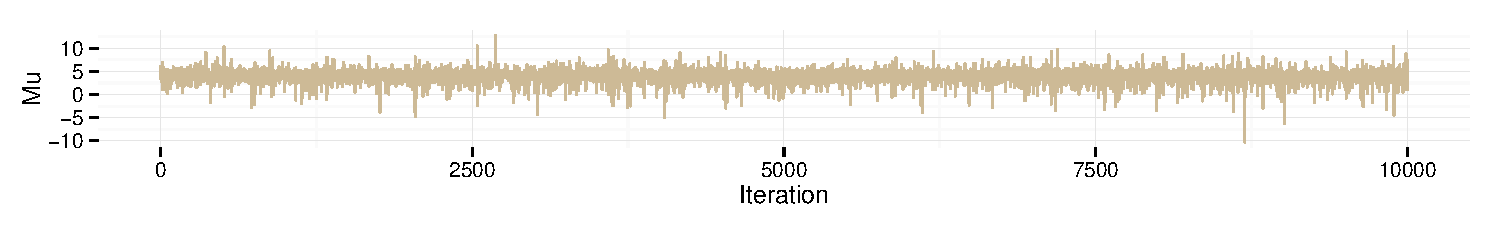
\includegraphics{markdown_hw3_files/figure-latex/unnamed-chunk-7-1.pdf}
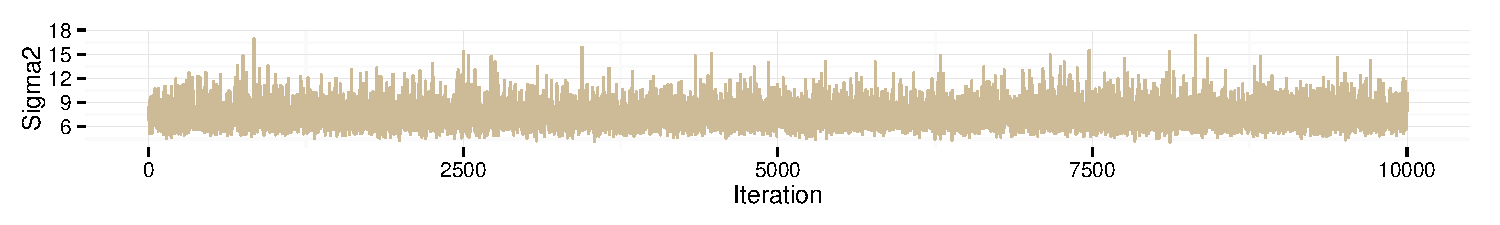
\includegraphics{markdown_hw3_files/figure-latex/unnamed-chunk-8-1.pdf}
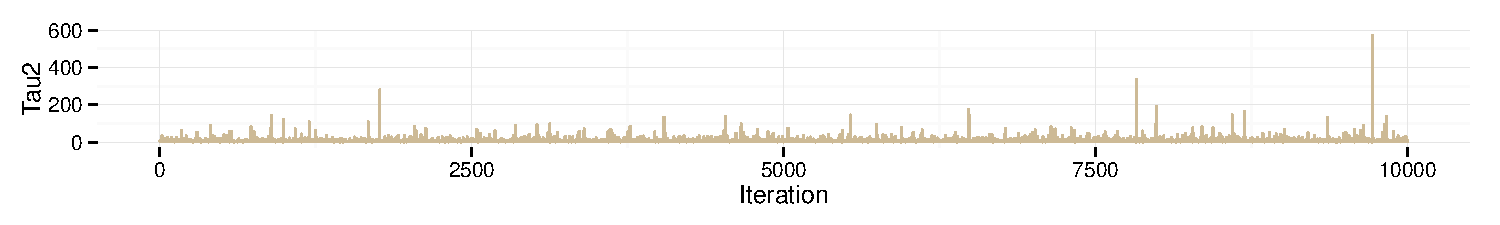
\includegraphics{markdown_hw3_files/figure-latex/unnamed-chunk-8-2.pdf}
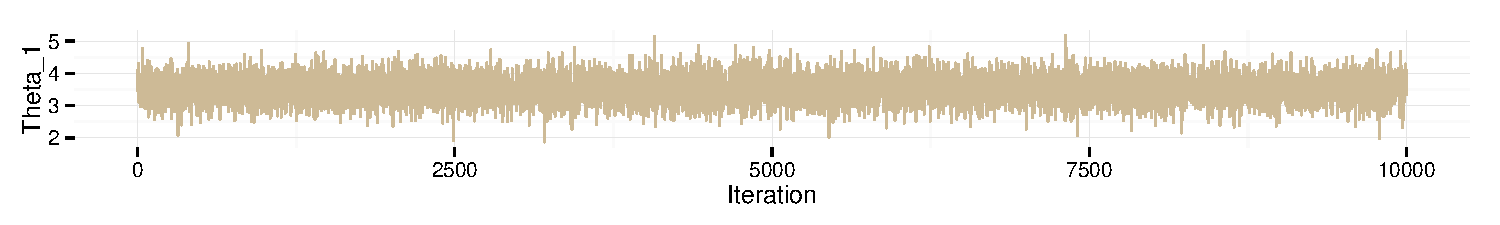
\includegraphics{markdown_hw3_files/figure-latex/unnamed-chunk-8-3.pdf}
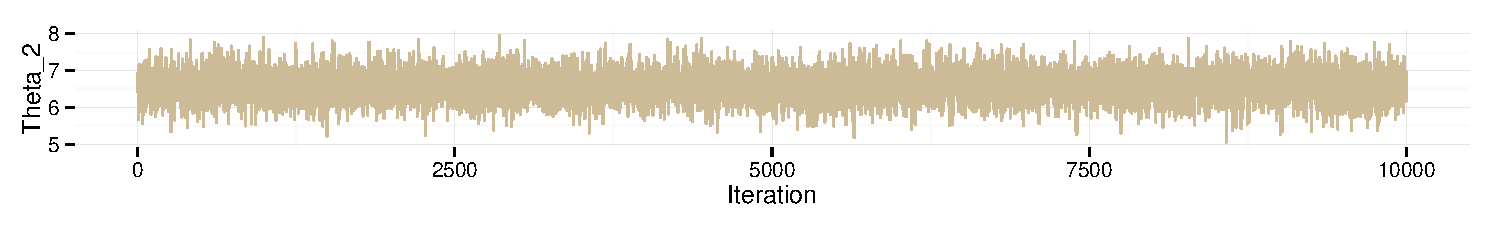
\includegraphics{markdown_hw3_files/figure-latex/unnamed-chunk-8-4.pdf}
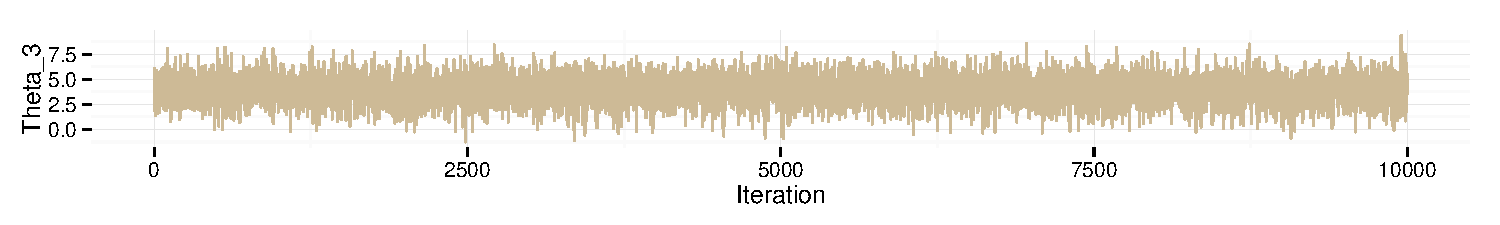
\includegraphics{markdown_hw3_files/figure-latex/unnamed-chunk-8-5.pdf}
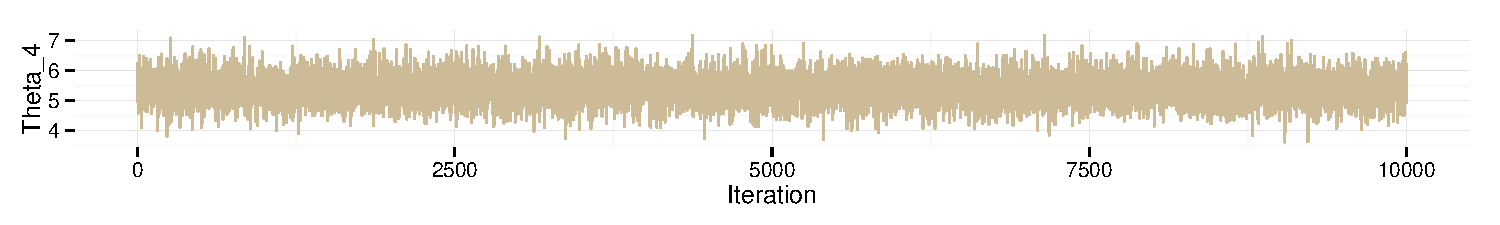
\includegraphics{markdown_hw3_files/figure-latex/unnamed-chunk-8-6.pdf}
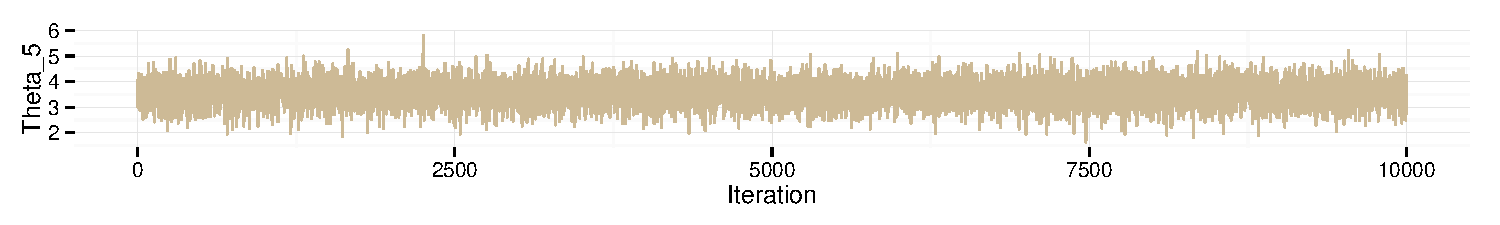
\includegraphics{markdown_hw3_files/figure-latex/unnamed-chunk-8-7.pdf}

We conclude from the graphs that convergence was achieved for all
parameters.

\subsection{1.3 Algorithm output}

The estimated median values and 95\% credible intervals for the
parameters are as follow:

\begin{Shaded}
\begin{Highlighting}[]
  \NormalTok{for(i in }\DecValTok{1}\NormalTok{:}\KeywordTok{length}\NormalTok{(ALL[}\DecValTok{1}\NormalTok{,])) }\KeywordTok{print}\NormalTok{(}\KeywordTok{round}\NormalTok{(}\KeywordTok{unname}\NormalTok{(}
    \KeywordTok{quantile}\NormalTok{(ALL[,i], }\DataTypeTok{probs=}\KeywordTok{c}\NormalTok{(}\FloatTok{0.025}\NormalTok{, }\FloatTok{0.5}\NormalTok{, }\FloatTok{0.975}\NormalTok{))}
    \NormalTok{),}\DecValTok{3}\NormalTok{))}
\end{Highlighting}
\end{Shaded}

\begin{center}
  \begin{tabular}{l c c c}
  \hline Parameter & Credible Lower 95\% & Median & Credible Upper 95\%  \\ \hline
    $\theta_1$ (Basmati) & 2.810 & 3.569 & 4.308 \\ 
    $\theta_2$ (Non-Basmati) & 5.790 & 6.533 & 7.305 \\
    $\theta_3$ (Beverage) & 1.869 & 4.231 & 6.448 \\
    $\theta_4$ (Cakes) & 4.486 & 5.370 & 6.301 \\
    $\theta_5$ (Cereal) & 2.705 & 3.610 & 4.507 \\
    $\mu$ & 3.193 & 4.697 & 6.182 \\
    $\sigma^2$ & 5.109 & 7.027 & 10.573 \\
    $\tau^2$ & 0.693 &2.251 & 12.920 \\ \hline
  \end{tabular}
\end{center}

\subsection{1.4 Sensitivity analyses}

Evaluation of sensitivity to priors: we try three separate scenarios
each tuning prior distribution of parameters:

\begin{enumerate}
  \item Large expected $\mu$ (Prior expectation of mad levels of arsenic)
  \item Large $\sigma^2$ and $\nu_0$ (High variability within products)
  \item Large $\tau^2$ and $\eta_0$ (High variability between products)
\end{enumerate}

Scenario 1:

\begin{center}
  \begin{tabular}{l c c c}
  \hline Parameter & Credible Lower 95\% & Median & Credible Upper 95\%  \\ \hline
    $\theta_1$ (Basmati)&2.706&3.488&4.265\\
    $\theta_2^2$ (Non-Basmati)&5.902&6.671&7.460\\
    $\theta_3 (Beverage)$&0.643&3.774&6.932\\
    $\theta_4 (Cakes)$&4.511&5.452&6.429\\
    $\theta_5$ (Cereal)&2.548&3.496&4.456\\
    $\mu$ &2.548&3.496&4.456\\
    $\sigma^2$ &88.793&100&111\\
    $\tau^2$ &3021.927&8427&37962\\ \hline
  \end{tabular}
\end{center}

Scenario 2:

\begin{center}
  \begin{tabular}{l c c c}
  \hline Parameter & Credible Lower 95\% & Median & Credible Upper 95\% \\ \hline
    $\theta_1$ (Basmati)& 1.237 & 4.396 & 7.069\\
    $\theta_2^2$ (Non-Basmati)& 2.811 & 5.401 & 8.559 \\
    $\theta_3 (Beverage)$& 0.278 & 4.790 & 9.023 \\
    $\theta_4 (Cakes)$& 1.931 & 4.960 & 8.221\\
    $\theta_5$ (Cereal)& 1.137 & 4.531 & 7.508\\
    $\mu$ &2.42 & 4.84 & 7.19\\
    $\sigma^2$ &182 & 215& 256\\
    $\tau^2$ &0.399 & 1.876 & 22.3\\ \hline

  \end{tabular}
\end{center}

Scenario 3:

\begin{center}
  \begin{tabular}{l c c c}
  \hline Parameter & Credible Lower 95\% & Median & Credible Upper 95\% \\ \hline
    $\theta_1$ (Basmati)& 2.707 & 3.478 & 4.268\\
    $\theta_2^2$ (Non-Basmati)& 5.907 & 6.674 & 7.451 \\
    $\theta_3 (Beverage)$& 0.676 & 3.739 & 6.9023 \\
    $\theta_4 (Cakes)$& 4.504 & 5.447 & 6.419\\
    $\theta_5$ (Cereal)& 2.547 & 3.494 & 4.452\\
    $\mu$ &-5.302 & 4.845 & 5.00\\
    $\sigma^2$ &5.197 & 7.327 & 11.37\\
    $\tau^2$ &223 & 288 & 384\\ \hline
  \end{tabular}
\end{center}

We observe that excessively large prior expectations of \(\mu\) will
drive estimates of the within- and between-group variances but will have
little effect on the magnitude of the estimates of within-groupmean
estimates (although the precision may be negatively affected for groups
with realtively few observations). A large prior within-sample variance
will bring posterior within-group means closer to \(\mu\), as could be
expected since the posterior estimates need to become more conservative.
Increasing prior between-sample variance appears to drive up uncertainty
on \(\mu\) and bring it closer to \(0\), without however having a
notable impact on the rest of the model.

\subsection{1.5 Results presentation}

Non-Basmati rice had the highest arsenic concentration, at an estimated
6.7 mcg/serving. Rice cakes came second, at 5.4 mcg/serving, and
non-Basmati and rice cereal had comparatively low amounts, slightly
below 3.5 mcg/serving. There lacked data to reliably evaluate arsenic
concentration in rice beverages, whose 3.8 mcg/serving estimate was
particulary imprecise (95\% CI=0.64, 6.93). Posterior median estimates
and observed mean concentrations of arsenic are presented by product
type in the following graph. Markers are \(\theta\) estimates with
\(95\%\) credible interval lines; horizontal lines are the median
estimate of \(\mu\) (solid) and corresponding \(95\%\) credibal interval
(dashed).

\begin{Shaded}
\begin{Highlighting}[]
\KeywordTok{library}\NormalTok{(plotrix)}
\NormalTok{qmat=}\KeywordTok{apply}\NormalTok{(THETA[,}\DecValTok{1}\NormalTok{:}\DecValTok{5}\NormalTok{],}\DecValTok{2}\NormalTok{,quantile,}\DataTypeTok{probs=}\KeywordTok{c}\NormalTok{(}\FloatTok{0.025}\NormalTok{,.}\DecValTok{5}\NormalTok{,}\FloatTok{0.975}\NormalTok{))}
\NormalTok{mu_ci =}\StringTok{ }\KeywordTok{quantile}\NormalTok{(OTH[,}\DecValTok{1}\NormalTok{], }\DataTypeTok{probs=}\NormalTok{(}\KeywordTok{c}\NormalTok{(}\FloatTok{0.025}\NormalTok{, }\FloatTok{0.5}\NormalTok{, }\FloatTok{0.975}\NormalTok{)))}
\NormalTok{res <-}\StringTok{ }\KeywordTok{data.frame}\NormalTok{(}\StringTok{"Rice"}\NormalTok{=}\KeywordTok{c}\NormalTok{(}\StringTok{"Non-Basmati"}\NormalTok{, }\StringTok{"Basmati"}\NormalTok{, }\StringTok{"Beverages"}\NormalTok{, }\StringTok{"Cakes"}\NormalTok{, }\StringTok{"Cereal"}\NormalTok{),}
                         \StringTok{"l95"}\NormalTok{=qmat[}\DecValTok{1}\NormalTok{,], }\StringTok{"median"}\NormalTok{=qmat[}\DecValTok{2}\NormalTok{,], }\StringTok{"u95"}\NormalTok{=qmat[}\DecValTok{3}\NormalTok{,])}
\NormalTok{g <-}\StringTok{ }\KeywordTok{ggplot}\NormalTok{(res, }\KeywordTok{aes}\NormalTok{(}\DataTypeTok{x =} \NormalTok{Rice, }\DataTypeTok{group=}\NormalTok{Rice, }\DataTypeTok{colour=}\NormalTok{Rice)) +}\StringTok{ }
\StringTok{  }\KeywordTok{labs}\NormalTok{(}\DataTypeTok{x=}\StringTok{"Rice Products"}\NormalTok{, }\DataTypeTok{y=}\StringTok{"Arsenic concentration, mcg/serving"}\NormalTok{) +}\StringTok{ }
\StringTok{  }\KeywordTok{theme}\NormalTok{(}\DataTypeTok{legend.position=}\StringTok{"none"}\NormalTok{, }\DataTypeTok{panel.background =}\KeywordTok{element_rect}\NormalTok{(}\DataTypeTok{colour =} \StringTok{"black"}\NormalTok{)) +}
\StringTok{  }\KeywordTok{scale_y_continuous}\NormalTok{(}\DataTypeTok{breaks=}\KeywordTok{seq}\NormalTok{(}\DecValTok{0}\NormalTok{, }\FloatTok{7.5}\NormalTok{, }\DecValTok{1}\NormalTok{)) +}
\StringTok{  }\KeywordTok{geom_hline}\NormalTok{(}\KeywordTok{aes}\NormalTok{(}\DataTypeTok{yintercept=}\KeywordTok{c}\NormalTok{(mu_ci[}\DecValTok{2}\NormalTok{])), }\DataTypeTok{size=}\FloatTok{0.7}\NormalTok{) +}
\StringTok{  }\KeywordTok{geom_hline}\NormalTok{(}\KeywordTok{aes}\NormalTok{(}\DataTypeTok{yintercept=}\KeywordTok{c}\NormalTok{(mu_ci[}\DecValTok{1}\NormalTok{])), }\DataTypeTok{linetype=}\StringTok{"dashed"}\NormalTok{) +}
\StringTok{  }\KeywordTok{geom_hline}\NormalTok{(}\KeywordTok{aes}\NormalTok{(}\DataTypeTok{yintercept=}\KeywordTok{c}\NormalTok{(mu_ci[}\DecValTok{3}\NormalTok{])), }\DataTypeTok{linetype=}\StringTok{"dashed"}\NormalTok{) +}
\StringTok{  }\KeywordTok{geom_errorbar}\NormalTok{(}\KeywordTok{aes}\NormalTok{(}\DataTypeTok{ymin=}\NormalTok{l95, }\DataTypeTok{ymax=}\NormalTok{u95), }\DataTypeTok{width=}\NormalTok{.}\DecValTok{3}\NormalTok{, }\DataTypeTok{size=}\FloatTok{0.8}\NormalTok{) +}
\StringTok{  }\KeywordTok{geom_point}\NormalTok{(}\KeywordTok{aes}\NormalTok{(}\DataTypeTok{y=}\NormalTok{median), }\DataTypeTok{fill=}\StringTok{"white"}\NormalTok{, }\DataTypeTok{shape=}\DecValTok{21}\NormalTok{, }\DataTypeTok{size=}\DecValTok{5}\NormalTok{) }
\NormalTok{g}
\end{Highlighting}
\end{Shaded}

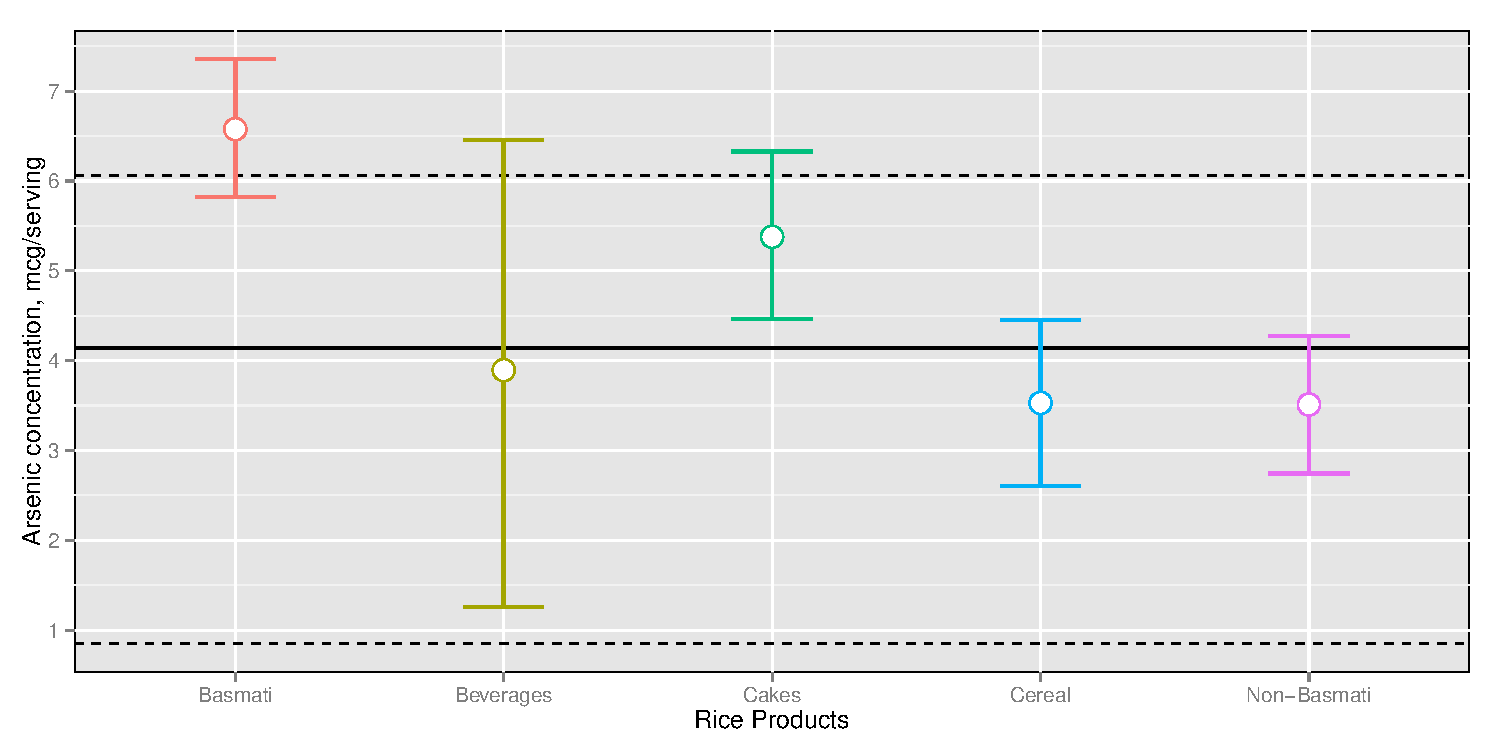
\includegraphics{markdown_hw3_files/figure-latex/unnamed-chunk-10-1.pdf}

\end{document}
